\documentclass[12pt]{article}

%%%%%%%%%%%%%%%%%%%%%%%%%%%%%%%%%%%%%%%%%%%%%%%%%%%%%%%%%%%%%%%%%%%%%%%%%%%%%%%%
%                           Package preset for homework
%%%%%%%%%%%%%%%%%%%%%%%%%%%%%%%%%%%%%%%%%%%%%%%%%%%%%%%%%%%%%%%%%%%%%%%%%%%%%%%%
% Miscellaneous
\usepackage[margin=1in]{geometry}
\usepackage[utf8]{inputenc}
\usepackage{indentfirst}
\usepackage{blindtext}
\usepackage{graphicx}
\usepackage{xr-hyper}
\usepackage{hyperref}
\usepackage{enumitem}
\usepackage{color}
\usepackage{float}
% Math
\usepackage{latexsym}
\usepackage{amsfonts}
\usepackage{amssymb}
\usepackage{amsmath}
\usepackage{commath}
\usepackage{amsthm}
\usepackage{bbold}
\usepackage{bm}
% Physics
\usepackage{physics}
\usepackage{siunitx}
% Code typesetting
\usepackage{listings}
% Citation
\usepackage[authoryear]{natbib}
\usepackage{appendix}
\usepackage[capitalize]{cleveref}
% Title & name
\title{Homework}
\author{Tien Vo}
\date{\today}


%%%%%%%%%%%%%%%%%%%%%%%%%%%%%%%%%%%%%%%%%%%%%%%%%%%%%%%%%%%%%%%%%%%%%%%%%%%%%%%%
%                   User-defined commands and environments
%%%%%%%%%%%%%%%%%%%%%%%%%%%%%%%%%%%%%%%%%%%%%%%%%%%%%%%%%%%%%%%%%%%%%%%%%%%%%%%%
%%% Misc
\sisetup{load-configurations=abbreviations}
\newcommand{\due}[1]{\date{Due: #1}}
\newcommand{\hint}{\textit{Hint}}
\let\oldt\t
\renewcommand{\t}[1]{\text{#1}}

%%% Bold sets & abbrv
\newcommand{\N}{\mathbb{N}}
\newcommand{\Z}{\mathbb{Z}}
\newcommand{\R}{\mathbb{R}}
\newcommand{\Q}{\mathbb{Q}}
\let\oldP\P
\renewcommand{\P}{\mathbb{P}}
\newcommand{\LL}{\mathcal{L}}
\newcommand{\FF}{\mathcal{F}}
\newcommand{\HH}{\mathcal{H}}
\newcommand{\NN}{\mathcal{N}}
\newcommand{\ZZ}{\mathcal{Z}}
\newcommand{\RN}[1]{\textup{\uppercase\expandafter{\romannumeral#1}}}
\newcommand{\ua}{\uparrow}
\newcommand{\da}{\downarrow}

%%% Unit vectors
\newcommand{\xhat}{\vb{\hat{x}}}
\newcommand{\yhat}{\vb{\hat{y}}}
\newcommand{\zhat}{\vb{\hat{z}}}
\newcommand{\nhat}{\vb{\hat{n}}}
\newcommand{\rhat}{\vb{\hat{r}}}
\newcommand{\phihat}{\bm{\hat{\phi}}}
\newcommand{\thetahat}{\bm{\hat{\theta}}}

%%% Other math stuff
\providecommand{\units}[1]{\,\ensuremath{\mathrm{#1}}\xspace}
% Set new style for problem
\newtheoremstyle{problemstyle}  % <name>
        {10pt}                   % <space above>
        {10pt}                   % <space below>
        {\normalfont}           % <body font>
        {}                      % <indent amount}
        {\bfseries\itshape}     % <theorem head font>
        {\normalfont\bfseries:} % <punctuation after theorem head>
        {.5em}                  % <space after theorem head>
        {}                      % <theorem head spec (can be left empty, 
                                % meaning `normal')>

% Set problem environment
\theoremstyle{problemstyle}
\newtheorem{problemenv}{Problem}[section]
\newenvironment{problem}[1]{%
  \renewcommand\theproblemenv{#1}%
  \problemenv
}{\endproblemenv}
% Set lemma environment
\newenvironment{lemma}[2][Lemma]{\begin{trivlist}
\item[\hskip \labelsep {\bfseries #1}\hskip \labelsep {\bfseries #2.}]}{\end{trivlist}}
% Set solution environment
\newenvironment{solution}{
    \begin{proof}[Solution]$ $\par\nobreak\ignorespaces
}{\end{proof}}
\numberwithin{equation}{problemenv}

%%% Page format
\setlength{\parindent}{0.5cm}
\setlength{\oddsidemargin}{0in}
\setlength{\textwidth}{6.5in}
\setlength{\textheight}{8.8in}
\setlength{\topmargin}{0in}
\setlength{\headheight}{18pt}

%%% Code environments
\definecolor{dkgreen}{rgb}{0,0.6,0}
\definecolor{gray}{rgb}{0.5,0.5,0.5}
\definecolor{mauve}{rgb}{0.58,0,0.82}
\lstset{frame=tb,
  language=Python,
  aboveskip=3mm,
  belowskip=3mm,
  showstringspaces=false,
  columns=flexible,
  basicstyle={\small\ttfamily},
  numbers=none,
  numberstyle=\tiny\color{gray},
  keywordstyle=\color{blue},
  commentstyle=\color{dkgreen},
  stringstyle=\color{mauve},
  breaklines=true,
  breakatwhitespace=true,
  tabsize=4
}
\lstset{
  language=Mathematica,
  numbers=left,
  numberstyle=\tiny\color{gray},
  numbersep=5pt,
  breaklines=true,
  captionpos={t},
  frame={lines},
  rulecolor=\color{black},
  framerule=0.5pt,
  columns=flexible,
  tabsize=2
}


\title{Homework 4: Phys 7230 (Spring 2022)}
\due{March 7, 2022}

\begin{document}
\maketitle
%%%%%%%%%%%%%%%%%%%%%%%%%%%%%%%%%%%%%%%%%%%%%%%%%%%%%%%%%%%%%%%%%%%%%%%%%%%%%%%
\begin{problem}{1}[Variational approximation]
In the lectures we derived the classical variational bound for the free energy,
given by
\begin{equation}
    F\leq F_\t{tr}+\expval{\HH-\HH_\t{tr}}_\t{tr}, 
\end{equation}
where $H_\t{tr}$ is the variational trial Hamiltonian that best approximates
$\HH$. To prove this result we utilize the convexity of a decaying exponential
function, namely for a random variable $x$<
\begin{equation}\label{p1:var_ineq}
    \expval{e^{-x}}\geq e^{-\expval{x}}. 
\end{equation}

(a) Prove above convexity inequality at least to lowest order in Taylor series
expansion.
\begin{solution}
\end{solution}

(b) Show that the variational inequality \eqref{p1:var_ineq} is equivalent to
$F\leq F_\t{v}=\expval{\HH}_\t{tr}-TS_\t{tr}$, where $S_\t{tr}$ is the Shannon's
entropy for the probability distribution $P=Z_\t{tr}^{-1}e^{-\beta\HH_\t{tr}}$,
with an extra factor of $k_B$ to make units consistent with our thermodynamics.
\begin{solution}
    
\end{solution}

(c) Consider a particle in a periodic potential described by a Hamiltonian
\begin{equation}
    \HH=\frac{p^2}{2m}+\alpha(1-\cos x), 
\end{equation}
where I took $x$ to be dimensionless, i.e., measured in units of another length
$x_0$ to simplify the notation. Motivated by the physical expectation that at
low $T$, a particle that starts at $x=0$ may be trapped in the minimum of the
cosine, use $\HH_\t{tr}=(1/2)kx^2$ to treat this problem variationally.

Specifically, please use the variational procedure to get an implicit equation
for the variational parameter function $k(\alpha/k_BT)$. Then solve this
equation for the function $k(\alpha/k_BT)$ numerically and/or graphically,
giving its two limits, the critical value of $(\alpha/k_BT)_c$ at which the
transition occurs, and sketching the function. You will find Mathematica useful.

\textit{Hint}: (1) You will find our Gaussian integral calculus very useful. (2)
You will obtain an implicit equation for the variational parameter $k$. You can
solve this equation numerically or graphically finding the behavior of
$k(\alpha/k_BT)$. From this solution show that the variational theory predicts a
phase transition in this problem in the solution for $k$ as a function of
$\alpha/k_BT$, namely that the thermodynamics (free energy, etc) has two
distinct phases, corresponding to high and low $\alpha/k_BT$. Just for the
record, this intriguing finding is an example of a failure of the variational
approximation for this single particle (0d) problem, that will, however, become
correct for higher dimensional problem, e.g., an extended $d$-dimensional
($d>1$) object, e.g., a fluctuating membrane trapped in a periodic potential.
\end{problem}
\newpage
%%%%%%%%%%%%%%%%%%%%%%%%%%%%%%%%%%%%%%%%%%%%%%%%%%%%%%%%%%%%%%%%%%%%%%%%%%%%%%%    

%%%%%%%%%%%%%%%%%%%%%%%%%%%%%%%%%%%%%%%%%%%%%%%%%%%%%%%%%%%%%%%%%%%%%%%%%%%%%%%
\begin{problem}{2}[Propagation in imaginary time, random walk and phantom
    polymer]

(a) Using Gaussian integral calculus demonstrate an important and very useful
(e.g., for path integrals and our applications below) Gaussians ``propagation''
relation,
\begin{equation}\label{p2a:prop_rel}
    \int_{-\infty}^\infty
    dx_2\frac1{\sqrt{2\pi\tau_2}}e^{-\frac{(x_3-x_2)^2}{2\tau_2}}
    \frac1{\sqrt{2\pi\tau_1}}e^{-\frac{(x_2-x_1)^2}{2\tau_1}}
    =\frac1{\sqrt{2\pi(\tau_2+\tau_1)}}e^{-\frac{(x_3-x_1)^2}{2(\tau_2+\tau_1)}},
\end{equation}
and thereby prove unnormalized density matrix the ``propagator'' property for
the \textit{free-particle},
\begin{equation}
    \rho^u(x_3,x_1;\tau_1+\tau_2)
    =\int dx_2\rho^u(x_3,x_2;\tau_2)\rho^u(x_2,x_1;\tau_1),
\end{equation}
that, as discussed in class is satisfied by all $\rho^u(x,x',\tau)$.
\begin{solution}
\end{solution}

(b) Edward's ``phantom'' polymer model, coupled harmonic oscillators, and a
random walk

As we may discuss in more detail in a few lectures, a simplest model of a
polymer (a giant flexible linear molecule of $N$ monomers strung together,
illutrated in \cref{fig:p2b} below) is that of a freely-joined chain of $N$
links $\vb{r}_n=\vb{R}_n-\vb{R}_{n-1}$. In the continuum, $n\to s$, the
probability of its conformation $\vb{R}(s)$ in a $d$-dimensional space is given
by
\begin{equation}
    P\qty[\vb{R}(s)]=\qty(\frac{d}{2\pi b_0^2})^{dN/2}
    \exp\qty[-\frac{d}{2b_0^2}\int_0^N ds\qty(\frac{\partial\vb{R}}{\partial
        s})^2],
\end{equation}
where $b_0$ is the preferred link length and prefactor is a normalization, much
like in \cref{p2a:prop_rel} for 2 links. We can view this system as described by
an ideal polymer Hamiltonian

\begin{figure}
    \centering
    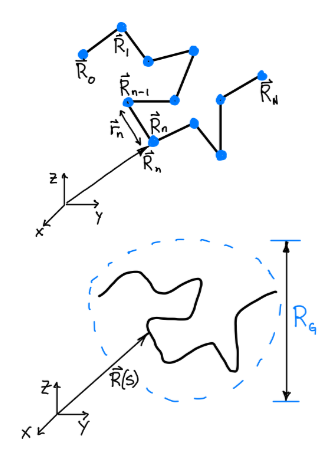
\includegraphics[width=0.4\textwidth]{p2b.png}
    \caption{Edward's ``phantom'' polymer model executing an ideal random walk
    in $d$-dimensional space, characterized by $N+1$ monomer positions,
$\vb{R}_n$.}
\label{fig:p2b}
\end{figure}

\begin{equation}
    \HH=\frac\sigma2\int_0^Nds\qty(\frac{\partial\vb{R}}{\partial s})^2,  
\end{equation}
where $\sigma=k_BTd/(\pi b_0^2)$ is the entropic polymer free energy per unit of
length, i.e., tension, notably proportional to thermal energy $k_BT$.

\qquad(i) By discretizing above probability distribution into product of $N$
1-link probability distributions,
\begin{equation}
    p(\vb{r}_n)=\qty(\frac{d}{2\pi b_0^2})^{d/2}
    \exp\qty[-\frac{d}{2b_0^2}\qty(\vb{R}_n-\vb{R}_{n-1})^2],
\end{equation}
written in terms of the position $\vb{R}_n$ of $n$-th monomer, and by
integrating over all $N$ \textit{intermediate} monomer positions, $\vb{R}_n$ for
$1<n<N$ compute the probability distribution $P\qty[\vb{R}_N-\vb{R}_0]$, for the
end-to-end displacement $\vb{R}_N-\vb{R}_0$.

\textit{Hint}: Surprise! You have just computed a path-integral for a single
polymer statistical mechanics, computing its partition function
$Z=\exp\qty(-\beta F)$, for fixed ends $\vb{R}_N,\vb{R}_0$ of the polymer.
\begin{solution}
    
\end{solution}

\qquad(ii) Compute the ``radius of gyration'' $R_g(N)$, defined by
\begin{equation}
    R_g^2=\expval{\qty(\vb{R}_N-\vb{R}_0)^2}, 
\end{equation}
which characterizes the root-mean-squared radius occupied by a polymer in the
$d$-dimensional embedding space.

Note that, in thinking of the links of the polymer as random steps executed as a
function of ``time'' $s$, this polymer statistics reproduces the random walk
result that after $N$ steps the random walker is only $\sqrt{N}$ away from where
she started. All this is of course a consequence of central limit theorem.

\begin{solution}
    
\end{solution}
\end{problem}
\newpage
%%%%%%%%%%%%%%%%%%%%%%%%%%%%%%%%%%%%%%%%%%%%%%%%%%%%%%%%%%%%%%%%%%%%%%%%%%%%%%%
%%%%%%%%%%%%%%%%%%%%%%%%%%%%%%%%%%%%%%%%%%%%%%%%%%%%%%%%%%%%%%%%%%%%%%%%%%%%%%%
\begin{problem}{3}[Free particle density matrix in coordinate representation]
In lectures we discussed many properties and forms of the coordinate-space
density matrix $\rho(x,x';\beta)$, including its expected low- and high-$T$
limits, as well as its eigenstates
\begin{equation}\label{p3:H_basis}
    \rho^u(x,x';\beta)=\sum_n\psi_n(x)\psi_n^\ast(x')e^{-\beta E_n},
\end{equation}
and path-integral
\begin{equation}\label{p3:path_int}
    \rho^u(x,x';\beta)=\int_{x(0)=x;x(\beta\hbar)=x'}\qty[dx(\tau)]
    e^{-S_E\qty[x(\tau)]/\hbar}
\end{equation}
formulations, as well as the ``imaginary-time'' Schr\"{o}dinger-like equation in
$\beta$
\begin{equation}\label{p3:Schrodinger_eq}
    \partial_\beta\rho^u(x,x';\beta)=-\HH\qty(\hat\rho,x)\rho^u(x,x';\beta), 
\end{equation}
that it satisfies, where $\hat\rho=-i\hbar\partial_x$, i.e., giving the
coordinate representation Schr\"{o}dinger equation in imaginary time. Let us
explore the details of this for a free particle here.

(a) For a free particle, use its Hamiltonian inside \eqref{p3:Schrodinger_eq},
solve the resulting diffusion equation (in ``time'' $\beta$) solve, taking into
account the appropriate ``initial condition''  for $\beta=0$, discussed in
class, required by the general definition of $\hat\rho^u$.

\textit{Hint}: The solution is as simple as solving free-particle
Schr\"{o}dinger equation in imaginary ``time'' or a real diffusion equation in
infinite space.
\begin{solution}
\end{solution}

(b) Use Hamiltonian eigenbasis representation, \cref{p3:H_basis} and your
knowledge of what the free-particle eigenstates are, to rederive the above
result for $\rho^u(x,x';\beta),$ also quoted in the lectures. Note that if you
properly take the eigenstates to be normalized in a large box of size $L$ (most
convenient with periodic boundary conditions), this analysis automatically gives
the correct prefactor for $\rho^u(x,x';\beta)$.
\begin{solution}
    
\end{solution}

(c) Now we will use, perhaps a bit less familiar path-integral formulation. One
useful approach to evaluate a path-integral is that of a semi-classical
saddle-point approximation.

\begin{itemize}
    \item An amazing fact, however, that we will see below is that this
        semi-classical approach is in fact \textit{exact} for a quadratic
        action, as for e.g.,, a free particle and harmonic oscillator (the
        following problem).
    \item Examining \cref{p3:path_int}, we see that all dependence of
        $\rho^u(x,x';\beta)$ on $x,x'$ is in the boundary conditions on
        $x(0),x(\beta\hbar)$. So let's introduce new time-dependent coordinates
        $y(\tau)$, with
        \begin{equation}\label{p3c:new_x}
            x(\tau)=x_\t{cl}(\tau)+y(\tau), 
        \end{equation}
        where $x_\t{cl}(\tau)$ is the classical path satisfying the
        Euler-Lagrange equation
        \begin{equation}\label{p3c:eom}
            \eval{\frac{\delta S_E\qty[x(\tau)]}{\delta
            x(\tau)}}_{x_\t{cl}(\tau)}=0, 
        \end{equation}
        and satisfying $x_\t{cl}(0)=x,x_\t{cl}(\beta\hbar)=x'$. Thus,
        $y(0)=y(\beta\hbar)=0$.

    \item Inserting \cref{p3c:new_x} into the action in \cref{p3:path_int} and
        expanding to lowest nontrivial order in $y(\tau)$ we find
        \begin{equation}\label{p3c:approx_dens_matrix}
            \rho^u(x,x';\beta)\approx
            e^{-S_E\qty[x_\t{cl}(\tau)]/\hbar}
            \int_{y(0)=y(\beta\hbar)=0}\qty[dy(\tau)]
            \exp\qty[-\frac1{2\hbar}\int_0^{\beta\hbar}d\tau
            y(\tau)S_E''[x_\t{cl}]y(\tau)],
        \end{equation}
        where first functional derivative term is absent because it vanishes by
        virtue of the equation of motion \cref{p3c:eom} satisfied by 
        $x_\t{cl}(\tau)$.

    \item The key observation in \cref{p3c:approx_dens_matrix} is that for
        quadratic action $S_E\qty[x(\tau)]$, the kernel $S_E''\qty[x_\t{cl}]$
        in the exponential is independent of $x_\t{cl}(\tau)$. Thus, for such
        quadratic theory, the remaining functional integral over
        $y(\tau)\NN(\beta\hbar)$ is just a ``constant'' that only depends on
        $\beta\hbar$, but \textit{not} not on $x,x'$. We can therefore not worry
        about this prefactor $\NN(\beta\hbar)$ and focus on
        $\exp\qty(-S_E\qty[x_\t{cl}(\tau)]/\hbar)$ that contains all the key
        dependence on $x,x'$, giving us $\rho^u(x,x';\beta)$ up to the factor
        $\NN(\beta\hbar)$.
\end{itemize}

\begin{solution}
    
\end{solution}

(d) For a free particle, solve the (Euclidean) classical Euler-Lagrange equation
of motion \cref{p3c:eom} for $x(\tau,x,x')$ with initial conditions
$x_\t{cl}(0)=x,x_\t{cl}(\beta\hbar)=x'$, and evaluate
\begin{equation}
    S_E\qty[x_\t{cl}(\tau)]\equiv S_\t{cl}(x,x',\beta\hbar), 
\end{equation}
thereby obtaining
\begin{equation}\label{p3d:dens_matrix}
    \rho^u(x,x';\beta)=\NN(\beta\hbar)e^{-S_\t{cl}(x,x',\beta\hbar)/\hbar}. 
\end{equation}
Demonstrate that up to the unknown prefactor $\NN(\beta\hbar)$, you obtain
exactly the result found in (a) and (b).
\begin{solution}
    
\end{solution}

(e) As a non-required bonus, you can determine the prefactor $\NN(\beta\hbar)$,
by discretizing the path integral in \eqref{p3c:approx_dens_matrix} as you did
for a polymer in problem 2 (note mathematically it is exactly the same path
integral) and then requiring the $\NN(\Delta\tau)$ (with
$\beta\hbar=N\Delta\tau)$ to be special function such that the ``propagator''
relation, \eqref{p2:prop_rel} is satisfied.

Alternatively,you can determine $\NN(\tau)$ by requiring that
\eqref{p3d:dens_matrix} satisfies the diffusion equation,
\eqref{p3:Schrodinger_eq}, thereby obtaining and solving a differential equation
for $\NN(\tau)$.
\begin{solution}
    
\end{solution}

(f) Now that we have obtained $\rho^u(x,x';\beta)$ by three methods above,
calculate the corresponding (i) partition function $Z(\beta)$ and the (ii)
probability $P(x)=\rho^u(x,x,\beta)/Z(\beta)$ of finding a free particle at
position $x$.

\textit{Hint}: The answer makes sense and is trivial.

\end{problem}
\newpage
%%%%%%%%%%%%%%%%%%%%%%%%%%%%%%%%%%%%%%%%%%%%%%%%%%%%%%%%%%%%%%%%%%%%%%%%%%%%%%%
\end{document}
